\documentclass[12pt]{article}

\usepackage{geometry}
\geometry{a4paper, left=1in, right=1in, top=1in, bottom=1in}
\usepackage{amsmath}
\usepackage{amsmath,amsfonts,amssymb}
\usepackage{graphicx}
\usepackage{enumitem}
\usepackage{titlesec}
\usepackage{fancyhdr}
\usepackage{hyperref}
\usepackage{floatrow}
\usepackage{geometry}
\usepackage{fancyhdr}
\usepackage{empheq}
\usepackage[svgnames]{xcolor}
\usepackage{xpatch}

\makeatletter
\newcommand{\colorboxed}[1]{\fcolorbox{Black}{White}{\m@th$\displaystyle#1$}}
\xpatchcmd{\@Aboxed}{\boxed}{\colorboxed}{}{}
\makeatother
\usepackage{tikz}
\usepackage{subcaption}
\usetikzlibrary{quotes, angles, decorations.markings, intersections}
\usetikzlibrary{calc,patterns,angles,quotes, 3d, intersections, positioning, shapes, automata, positioning}
\usepackage{wasysym}
\title{{\bf CS663 Assignment 2}}
\author{Saksham Rathi, Kavya Gupta, Shravan Srinivasa Raghavan}
\date{September 2024}
\begin{document}
\maketitle
\clearpage
\tableofcontents
\clearpage
\section*{Question 4}
\addcontentsline{toc}{section}{Question 4}
    The derivate operators for 1D images are defined as follows:
    \begin{align*}
        \frac{df}{dx} &= f(x + 1) - f(x) \\
        \frac{d^{2}f}{dx^{2}} &= f(x + 1) + f(x - 1) - 2f(x) 
    \end{align*}

    Let us consider a 1D image and it's derivatives. The size of the image is 15 pixels for simplicity.

    \begin{figure}[H]
        \centering
        \begin{subfigure}[b]{\textwidth}
            \centering
            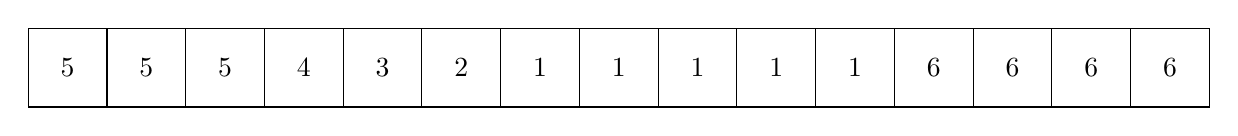
\begin{tikzpicture}
                \draw (-8,0) rectangle (7,1);
        
                \foreach \x in {-8,...,6}
                    \draw (\x+1,0) -- (\x+1,1);
        
                \node at (-7.5, 0.5) {5};
                \node at (-6.5, 0.5) {5};
                \node at (-5.5, 0.5) {5};
                \node at (-4.5, 0.5) {4};
                \node at (-3.5, 0.5) {3};
                \node at (-2.5, 0.5) {2};
                \node at (-1.5, 0.5) {1};
                \node at (-0.5, 0.5) {1};
                \node at (0.5, 0.5) {1};
                \node at (1.5, 0.5) {1};
                \node at (2.5, 0.5) {1};
                \node at (3.5, 0.5) {6};
                \node at (4.5, 0.5) {6};
                \node at (5.5, 0.5) {6};
                \node at (6.5, 0.5) {6};
            \end{tikzpicture}
            \caption{Image}
        \end{subfigure}
        
        \vspace{10pt}
        
        \begin{subfigure}[b]{\textwidth}
            \centering
            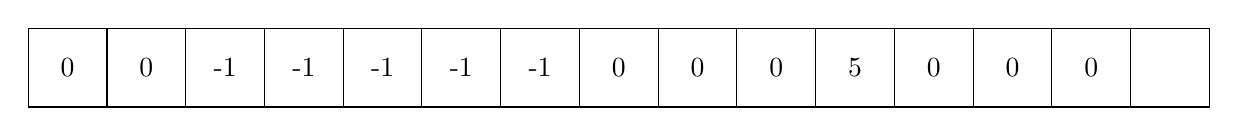
\begin{tikzpicture}
                \draw (-8,0) rectangle (7,1);
        
                \foreach \x in {-8,...,6}
                    \draw (\x+1,0) -- (\x+1,1);
        
                \node at (-7.5, 0.5) {0};
                \node at (-6.5, 0.5) {0};
                \node at (-5.5, 0.5) {-1};
                \node at (-4.5, 0.5) {-1};
                \node at (-3.5, 0.5) {-1};
                \node at (-2.5, 0.5) {-1};
                \node at (-1.5, 0.5) {-1};
                \node at (-0.5, 0.5) {0};
                \node at (0.5, 0.5) {0};
                \node at (1.5, 0.5) {0};
                \node at (2.5, 0.5) {5};
                \node at (3.5, 0.5) {0};
                \node at (4.5, 0.5) {0};
                \node at (5.5, 0.5) {0};
                \node at (6.5, 0.5) {};
            \end{tikzpicture}
            \caption{First derivatives}
        \end{subfigure}

        \vspace{10pt}
        
        \begin{subfigure}[b]{\textwidth}
            \centering
            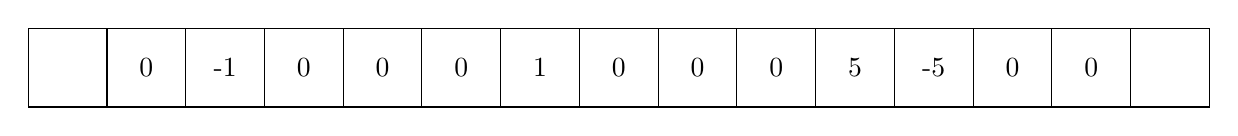
\begin{tikzpicture}
                \draw (-8,0) rectangle (7,1);
        
                \foreach \x in {-8,...,6}
                    \draw (\x+1,0) -- (\x+1,1);
        
                \node at (-7.5, 0.5) {};
                \node at (-6.5, 0.5) {0};
                \node at (-5.5, 0.5) {-1};
                \node at (-4.5, 0.5) {0};
                \node at (-3.5, 0.5) {0};
                \node at (-2.5, 0.5) {0};
                \node at (-1.5, 0.5) {1};
                \node at (-0.5, 0.5) {0};
                \node at (0.5, 0.5) {0};
                \node at (1.5, 0.5) {0};
                \node at (2.5, 0.5) {5};
                \node at (3.5, 0.5) {-5};
                \node at (4.5, 0.5) {0};
                \node at (5.5, 0.5) {0};
                \node at (6.5, 0.5) {};
            \end{tikzpicture}
            \caption{Second derivatives}
        \end{subfigure}
    \end{figure}
    Let us take $\alpha = 0.1$. For convenience we will drop the captions and have all three rows of data
    directly one below the other in the same order as before.
    After one iteration we have,
    \begin{figure}[H]
        \centering
        \begin{subfigure}[b]{\textwidth}
            \centering
            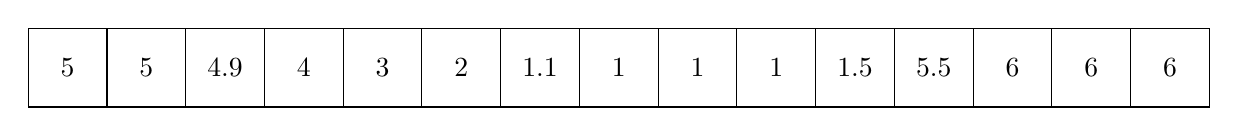
\begin{tikzpicture}
                \draw (-8,0) rectangle (7,1);
        
                \foreach \x in {-8,...,6}
                    \draw (\x+1,0) -- (\x+1,1);
        
                \node at (-7.5, 0.5) {5};
                \node at (-6.5, 0.5) {5};
                \node at (-5.5, 0.5) {4.9};
                \node at (-4.5, 0.5) {4};
                \node at (-3.5, 0.5) {3};
                \node at (-2.5, 0.5) {2};
                \node at (-1.5, 0.5) {1.1};
                \node at (-0.5, 0.5) {1};
                \node at (0.5, 0.5) {1};
                \node at (1.5, 0.5) {1};
                \node at (2.5, 0.5) {1.5};
                \node at (3.5, 0.5) {5.5};
                \node at (4.5, 0.5) {6};
                \node at (5.5, 0.5) {6};
                \node at (6.5, 0.5) {6};
            \end{tikzpicture}
        \end{subfigure}
        
        
        \begin{subfigure}[b]{\textwidth}
            \centering
            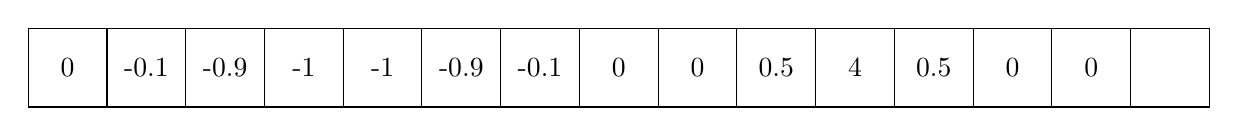
\begin{tikzpicture}
                \draw (-8,0) rectangle (7,1);
        
                \foreach \x in {-8,...,6}
                    \draw (\x+1,0) -- (\x+1,1);
        
                \node at (-7.5, 0.5) {0};
                \node at (-6.5, 0.5) {-0.1};
                \node at (-5.5, 0.5) {-0.9};
                \node at (-4.5, 0.5) {-1};
                \node at (-3.5, 0.5) {-1};
                \node at (-2.5, 0.5) {-0.9};
                \node at (-1.5, 0.5) {-0.1};
                \node at (-0.5, 0.5) {0};
                \node at (0.5, 0.5) {0};
                \node at (1.5, 0.5) {0.5};
                \node at (2.5, 0.5) {4};
                \node at (3.5, 0.5) {0.5};
                \node at (4.5, 0.5) {0};
                \node at (5.5, 0.5) {0};
                \node at (6.5, 0.5) {};
            \end{tikzpicture}
        \end{subfigure}
        
        \begin{subfigure}[b]{\textwidth}
            \centering
            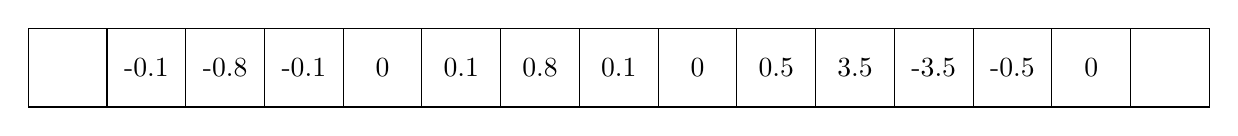
\begin{tikzpicture}
                \draw (-8,0) rectangle (7,1);
        
                \foreach \x in {-8,...,6}
                    \draw (\x+1,0) -- (\x+1,1);
        
                \node at (-7.5, 0.5) {};
                \node at (-6.5, 0.5) {-0.1};
                \node at (-5.5, 0.5) {-0.8};
                \node at (-4.5, 0.5) {-0.1};
                \node at (-3.5, 0.5) {0};
                \node at (-2.5, 0.5) {0.1};
                \node at (-1.5, 0.5) {0.8};
                \node at (-0.5, 0.5) {0.1};
                \node at (0.5, 0.5) {0};
                \node at (1.5, 0.5) {0.5};
                \node at (2.5, 0.5) {3.5};
                \node at (3.5, 0.5) {-3.5};
                \node at (4.5, 0.5) {-0.5};
                \node at (5.5, 0.5) {0};
                \node at (6.5, 0.5) {};
            \end{tikzpicture}
        \end{subfigure}
    \end{figure}
    Proceeding ahead we get,
    \begin{figure}[H]
        \centering
        \begin{subfigure}[b]{\textwidth}
            \centering
            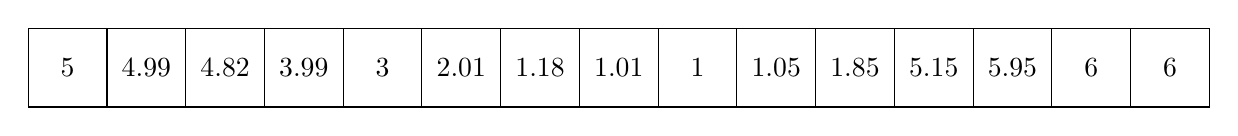
\begin{tikzpicture}
                \draw (-8,0) rectangle (7,1);
        
                \foreach \x in {-8,...,6}
                    \draw (\x+1,0) -- (\x+1,1);
        
                \node at (-7.5, 0.5) {5};
                \node at (-6.5, 0.5) {4.99};
                \node at (-5.5, 0.5) {4.82};
                \node at (-4.5, 0.5) {3.99};
                \node at (-3.5, 0.5) {3};
                \node at (-2.5, 0.5) {2.01};
                \node at (-1.5, 0.5) {1.18};
                \node at (-0.5, 0.5) {1.01};
                \node at (0.5, 0.5) {1};
                \node at (1.5, 0.5) {1.05};
                \node at (2.5, 0.5) {1.85};
                \node at (3.5, 0.5) {5.15};
                \node at (4.5, 0.5) {5.95};
                \node at (5.5, 0.5) {6};
                \node at (6.5, 0.5) {6};
            \end{tikzpicture}
        \end{subfigure}
        
        
        \begin{subfigure}[b]{\textwidth}
            \centering
            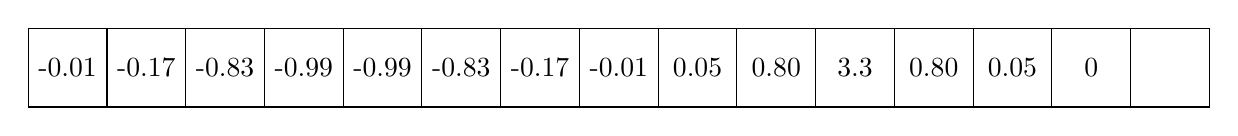
\begin{tikzpicture}
                \draw (-8,0) rectangle (7,1);
        
                \foreach \x in {-8,...,6}
                    \draw (\x+1,0) -- (\x+1,1);
        
                \node at (-7.5, 0.5) {-0.01};
                \node at (-6.5, 0.5) {-0.17};
                \node at (-5.5, 0.5) {-0.83};
                \node at (-4.5, 0.5) {-0.99};
                \node at (-3.5, 0.5) {-0.99};
                \node at (-2.5, 0.5) {-0.83};
                \node at (-1.5, 0.5) {-0.17};
                \node at (-0.5, 0.5) {-0.01};
                \node at (0.5, 0.5) {0.05};
                \node at (1.5, 0.5) {0.80};
                \node at (2.5, 0.5) {3.3};
                \node at (3.5, 0.5) {0.80};
                \node at (4.5, 0.5) {0.05};
                \node at (5.5, 0.5) {0};
                \node at (6.5, 0.5) {};
            \end{tikzpicture}
        \end{subfigure}
        
        \begin{subfigure}[b]{\textwidth}
            \centering
            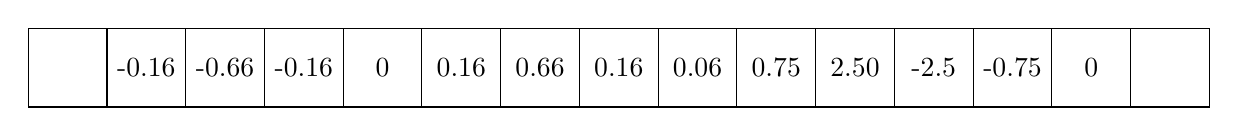
\begin{tikzpicture}
                \draw (-8,0) rectangle (7,1);
        
                \foreach \x in {-8,...,6}
                    \draw (\x+1,0) -- (\x+1,1);
        
                \node at (-7.5, 0.5) {};
                \node at (-6.5, 0.5) {-0.16};
                \node at (-5.5, 0.5) {-0.66};
                \node at (-4.5, 0.5) {-0.16};
                \node at (-3.5, 0.5) {0};
                \node at (-2.5, 0.5) {0.16};
                \node at (-1.5, 0.5) {0.66};
                \node at (-0.5, 0.5) {0.16};
                \node at (0.5, 0.5) {0.06};
                \node at (1.5, 0.5) {0.75};
                \node at (2.5, 0.5) {2.50};
                \node at (3.5, 0.5) {-2.5};
                \node at (4.5, 0.5) {-0.75};
                \node at (5.5, 0.5) {0};
                \node at (6.5, 0.5) {};
            \end{tikzpicture}
        \end{subfigure}
    \end{figure}
    Clearly, the intensities across edges are now closer than they were before the process ie the gradient across edges has reduced
    in magnitude.

    Running a \verb|MATLAB| script to do this resulted in the following images:
    \begin{enumerate}
        \item After a 100 iterations,
        \begin{figure}[H]
            \centering
                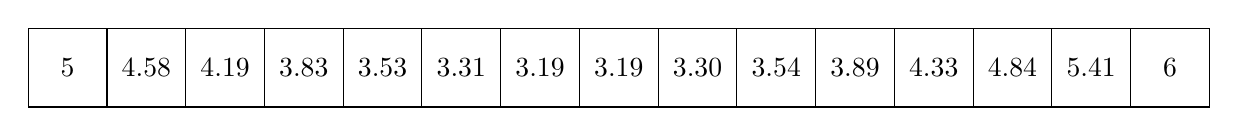
\begin{tikzpicture}
                    \draw (-8,0) rectangle (7,1);
            
                    \foreach \x in {-8,...,6}
                        \draw (\x+1,0) -- (\x+1,1);
            
                    \node at (-7.5, 0.5) {5};
                    \node at (-6.5, 0.5) {4.58};
                    \node at (-5.5, 0.5) {4.19};
                    \node at (-4.5, 0.5) {3.83};
                    \node at (-3.5, 0.5) {3.53};
                    \node at (-2.5, 0.5) {3.31};
                    \node at (-1.5, 0.5) {3.19};
                    \node at (-0.5, 0.5) {3.19};
                    \node at (0.5, 0.5) {3.30};
                    \node at (1.5, 0.5) {3.54};
                    \node at (2.5, 0.5) {3.89};
                    \node at (3.5, 0.5) {4.33};
                    \node at (4.5, 0.5) {4.84};
                    \node at (5.5, 0.5) {5.41};
                    \node at (6.5, 0.5) {6};
                \end{tikzpicture}
        \end{figure}

        \item After a 1000 iterations,
        \begin{figure}[H]
            \centering
                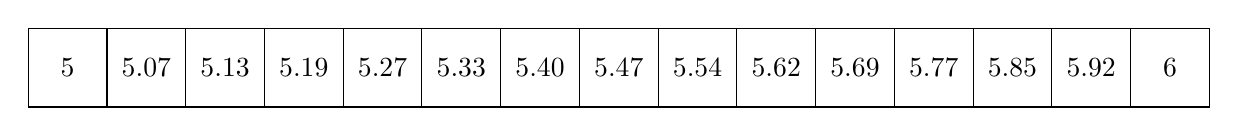
\begin{tikzpicture}
                    \draw (-8,0) rectangle (7,1);
            
                    \foreach \x in {-8,...,6}
                        \draw (\x+1,0) -- (\x+1,1);
            
                    \node at (-7.5, 0.5) {5};
                    \node at (-6.5, 0.5) {5.07};
                    \node at (-5.5, 0.5) {5.13};
                    \node at (-4.5, 0.5) {5.19};
                    \node at (-3.5, 0.5) {5.27};
                    \node at (-2.5, 0.5) {5.33};
                    \node at (-1.5, 0.5) {5.40};
                    \node at (-0.5, 0.5) {5.47};
                    \node at (0.5, 0.5) {5.54};
                    \node at (1.5, 0.5) {5.62};
                    \node at (2.5, 0.5) {5.69};
                    \node at (3.5, 0.5) {5.77};
                    \node at (4.5, 0.5) {5.85};
                    \node at (5.5, 0.5) {5.92};
                    \node at (6.5, 0.5) {6};
                \end{tikzpicture}
        \end{figure}
        \item After 10000 iterations,
        \begin{figure}[H]
            \centering
                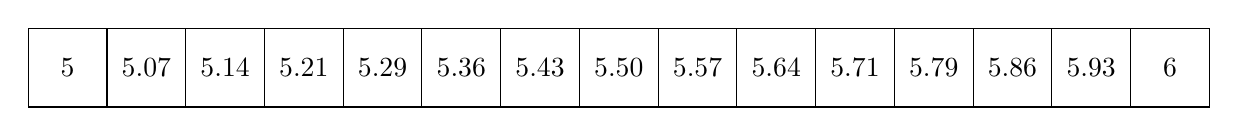
\begin{tikzpicture}
                    \draw (-8,0) rectangle (7,1);
            
                    \foreach \x in {-8,...,6}
                        \draw (\x+1,0) -- (\x+1,1);
            
                    \node at (-7.5, 0.5) {5};
                    \node at (-6.5, 0.5) {5.07};
                    \node at (-5.5, 0.5) {5.14};
                    \node at (-4.5, 0.5) {5.21};
                    \node at (-3.5, 0.5) {5.29};
                    \node at (-2.5, 0.5) {5.36};
                    \node at (-1.5, 0.5) {5.43};
                    \node at (-0.5, 0.5) {5.50};
                    \node at (0.5, 0.5) {5.57};
                    \node at (1.5, 0.5) {5.64};
                    \node at (2.5, 0.5) {5.71};
                    \node at (3.5, 0.5) {5.79};
                    \node at (4.5, 0.5) {5.86};
                    \node at (5.5, 0.5) {5.93};
                    \node at (6.5, 0.5) {6};
                \end{tikzpicture}
        \end{figure}
    \end{enumerate}
    Clearly, the intensities tend toward some local average value. This leads to blurring of the image.
    Earlier there were sharp intensitywe obtained the following results by running a \verb|MATLAB| scriptn which repeated this process for about $1000$ iterations:
    \begin{figure}[H]
        \centering
            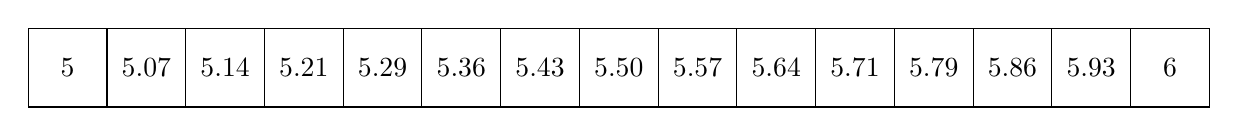
\begin{tikzpicture}
                \draw (-8,0) rectangle (7,1);
        
                \foreach \x in {-8,...,6}
                    \draw (\x+1,0) -- (\x+1,1);
        
                \node at (-7.5, 0.5) {5};
                \node at (-6.5, 0.5) {5.07};
                \node at (-5.5, 0.5) {5.14};
                \node at (-4.5, 0.5) {5.21};
                \node at (-3.5, 0.5) {5.29};
                \node at (-2.5, 0.5) {5.36};
                \node at (-1.5, 0.5) {5.43};
                \node at (-0.5, 0.5) {5.50};
                \node at (0.5, 0.5) {5.57};
                \node at (1.5, 0.5) {5.64};
                \node at (2.5, 0.5) {5.71};
                \node at (3.5, 0.5) {5.79};
                \node at (4.5, 0.5) {5.86};
                \node at (5.5, 0.5) {5.93};
                \node at (6.5, 0.5) {6};
            \end{tikzpicture}
    \end{figure} gradients denoting clear edges. Therefore, adding the term $\alpha \frac{d^{2}I(x)}{dx^{2}}$
    repeatedly causes blurring of edges resulting in a smooth image with intensities that are close in values throughout
    the image.

    In the case of 2D images, adding the term $\alpha \nabla^{2}I(x,y)$ to $I(x,y)$ achieves something similar. We can reason this
    as follows, clearly for every pixel $(x,y)$, there are only four immediate neighbours $(x - 1,y),(x + 1,y),(x,y - 1),(x,y + 1)$
    and therefore similar effects can be expected as the laplacian for 2D images takes the form
    \begin{align*}
        \nabla^{2} I(x,y) = I(x - 1,y) + I(x + 1,y) + I(x,y - 1) + I(x,y + 1) - 4I(x,y)
    \end{align*}

    So doing this for many iterations will result in every pixel tending towards some sort of average intensity of 
    it's neighbourhood resulting in a distribution where most intensities are close by in value.

    If, instead the term $\alpha \nabla^{2} I(x,y)$ were subtracted however, we get an image which is quite different. This 
    essentially increases the sharpness of the image and the range of intensities becomes wider resulting in an image where
    every edge is sharper ie higher gradients are found across edges. 
\end{document}